\chapter{¿Elevado o subterráneo? Conclusiones sobre el metro de Bogotá}\label{cap:metro}

La Primera Línea del Metro de Bogotá se construye sobre un viaducto. Una posición extendida en el debate
público sostiene que, por el tamaño de la ciudad, debió ser subterránea. Este capítulo trata esa
posición como una hipótesis y la somete al modelo con las dos fases de la investigación. La regla que
se sigue es dejar que el modelo decida y, donde la respuesta dependa de supuestos, mostrar con
precisión en qué punto cambia.

\section{Qué significa «por el tamaño de Bogotá»}

El argumento del tamaño puede leerse de tres formas, y cada una tiene una implicación distinta para la
tipología:
\begin{enumerate}[nosep]
\item \emph{Demanda}: una ciudad grande genera cargas por corredor que exigen alta capacidad. Esta
      lectura favorece al subterráneo solo si la capacidad del viaducto es insuficiente.
\item \emph{Tejido urbano}: una ciudad grande y densa tiene más gente y más valor inmobiliario junto a
      la línea, de modo que el costo urbano de un viaducto es mayor.
\item \emph{Red}: una ciudad grande necesita muchas líneas, no una. Esta lectura plantea la pregunta de
      cuántos kilómetros de metro se pueden construir con un presupuesto dado.
\end{enumerate}
Las secciones siguientes examinan cada una con los costos, el modelo de transporte y una estimación
del costo urbano del viaducto.

\section{Costos de las dos tipologías}\label{sec:costos_metro}

Para comparar tipologías con una sola fuente se usan los costos unitarios del estudio de la Empresa
Metro de 2023, que derivan de los precios de la concesión de la Línea 1 y de la estructuración de la
Línea 2 \citep{emb2023}. En pesos de noviembre de 2022, la obra civil cuesta 161.947 millones por
kilómetro en viaducto y 264.609 en túnel (63\,\% más); los sistemas y el material rodante, 241.043 y
284.257 millones por kilómetro; una estación, 129.742 millones elevada y 706.684 subterránea (5,4
veces), y la operación y el mantenimiento, 10.388 y 14.318 millones por kilómetro al año. Los costos
que no dependen de la tipología (patio-taller, predios, redes e interventoría) se toman iguales para
ambas. La \cref{tab:metro_costos} aplica esos unitarios, indexados a 2025, a cuatro trazados.

\begin{table}[ht]
\centering\small
\caption{CAPEX y O\&M de las tipologías elevada y subterránea con los costos unitarios de 2023
(billones de pesos de 2025, sin sobrecostos).}\label{tab:metro_costos}
\resizebox{\textwidth}{!}{\begin{tabular}{p{4.6cm}rrrrrrr}
\toprule
Línea & km & Est. & \multicolumn{2}{c}{CAPEX (billones)} & Prima & \multicolumn{2}{c}{O\&M (billones/año)} \\
\cmidrule(lr){4-5}\cmidrule(lr){7-8}
 & & & Elevado & Subterráneo & & Elevado & Subterráneo \\
\midrule
L1 (trazado elevado, 23,96 km) & 24,0 & 16 & 21,1 & 36,5 & 73\,\% & 0,30 & 0,41 \\
L1 subterránea 2014 (27 km) & 27,0 & 28 & 25,3 & 49,6 & 96\,\% & 0,34 & 0,47 \\
L2 (15,5 km) & 15,5 & 11 & 13,7 & 24,1 & 76\,\% & 0,19 & 0,27 \\
L3 (24,5 km) & 24,5 & 18 & 21,8 & 38,7 & 77\,\% & 0,31 & 0,42 \\
\bottomrule
\end{tabular}
}
\fuente{Costos unitarios de \citet{emb2023} indexados por \Indexacion; cálculos del autor.}
\end{table}

La prima del subterráneo es de \PrimaLuno{} para la Línea 1, \PrimaLdos{} para la Línea 2 y
\PrimaLtres{} para la Línea 3, y de casi 100\,\% para el trazado de 2014, que tenía más estaciones. En
términos de red, con el presupuesto de un kilómetro subterráneo se construyen \KmPorKm{} kilómetros
elevados. El costo oficial de 2014, reexpresado en pesos de 2025 (\CapexSubOficial{} billones), es
mucho menor que el que resulta de aplicar los unitarios a ese mismo trazado (\CapexSubUnitarios): la
diferencia refleja que aquel era un costo de ingeniería básica y estos son precios de mercado
posteriores. La verdad probablemente está entre ambos, y por eso los resultados se presentan con los
dos.

\section{Lo que gana y lo que pierde cada tipología}

\paragraph{A favor del subterráneo.} El túnel elimina el costo urbano del viaducto: ruido, sombra,
intrusión visual y efecto barrera. La evidencia hedónica muestra que ese costo existe y se concentra
cerca de la estructura. En Oslo, los precios de las viviendas aumentan con la distancia a la vía
férrea dentro de una franja de unos 100 metros \citep{strand2001}. En Berlín, \citet{ahlfeldt2016}
separan el efecto de accesibilidad de una línea de metro, que eleva el valor del suelo, del efecto del
ruido de los tramos elevados, que lo reduce; además, encuentran que el precio implícito del ruido se
triplicó en un siglo, con una elasticidad ingreso del valor de reducir el ruido de 2,2, y concluyen
que el argumento a favor de construir bajo tierra es hoy más fuerte que hace cien años
\citep{ahlfeldt2019}. El túnel da también libertad de trazado: puede pasar bajo zonas densas sin
avenidas anchas, donde un viaducto exigiría comprar predios.

\paragraph{A favor del elevado.} Cuesta mucho menos, se construye más rápido y opera más barato (el
O\&M por kilómetro del túnel es 38\,\% mayor, por ventilación, bombeo e iluminación). En los suelos
blandos de origen lacustre de buena parte de la Sabana, los túneles y las estaciones profundas tienen
un riesgo geotécnico que el modelo no diferencia: aplica a ambas tipologías la misma distribución de
sobrecostos, lo que favorece al subterráneo. Por último, el viaducto de la Línea 1 se apoya en
corredores anchos (la avenida Primero de Mayo y la Caracas), donde su costo urbano es menor que en un
tejido estrecho.

\section{Una estimación del costo urbano del viaducto}\label{sec:externalidad}

El modelo de transporte no valora el costo urbano del viaducto, pero puede preguntarse cuánto tendría
que valer para cambiar la decisión, y compararlo con una estimación independiente. La estimación se
basa en la pérdida de valor de los predios vecinos, con supuestos explícitos:
\begin{enumerate}[nosep]
\item Franja afectada: 100 m a cada lado de los 23,96 km del viaducto, es decir, 479 hectáreas, de las
      cuales el 65\,\% son lotes y el resto vías y espacio público.
\item Edificación: un índice de construcción de 1,5 a 2,5 sobre los lotes, es decir, entre 4,7 y 7,8
      millones de metros cuadrados construidos.
\item Valor: el promedio catastral de la ciudad, 919 billones de pesos sobre 307 millones de metros
      cuadrados construidos en 2025, unos 3,0 millones de pesos por metro cuadrado con el suelo incluido
      \citep{catastro2025}. El valor expuesto es de 14 a 23 billones.
\item Pérdida: entre 5\,\% y 10\,\% del valor, del orden de los efectos de proximidad y ruido de la
      literatura hedónica \citep{strand2001,ahlfeldt2019}.
\end{enumerate}
La pérdida capitalizada es de 0,7 a 2,3 billones, equivalente a un costo anual de 0,06 a 0,21 billones
con la tasa de 9\,\% y de 0,08 a 0,28 con la de 12\,\%. Si el valor comercial superara al catastral
en 50\,\%, el rango subiría hasta unos 0,4 billones por año. La medida tiene sesgos en ambas
direcciones: puede subestimar el costo, porque no capta el efecto barrera sobre quienes caminan o
atraviesan el corredor sin vivir en él, y puede sobreestimarlo, porque parte del ruido y de la sombra
se compensa con la renovación del espacio público que acompaña la obra.

\section{El mapa de decisión de la Primera Línea}

La \cref{fig:metro_decision} reúne los resultados de la fase I. Cada línea indica, para una tasa de
descuento, el costo urbano anual del viaducto que iguala las dos tipologías según el CAPEX del
subterráneo; por encima de la línea conviene el subterráneo y por debajo el elevado. La franja gris es
el rango estimado en la sección anterior.

\begin{figure}[ht]
\centering
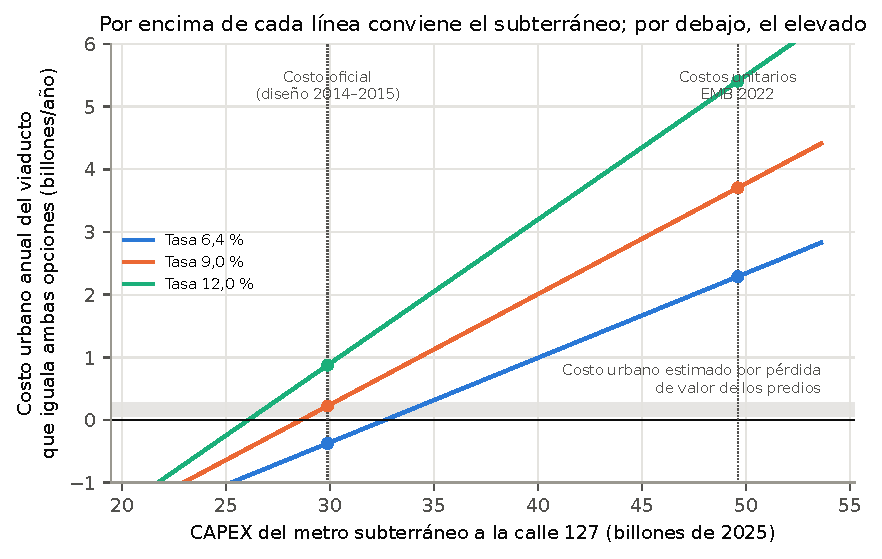
\includegraphics[width=.92\textwidth]{figuras/fig_metro_decision.pdf}
\caption{Mapa de decisión de la Primera Línea: costo urbano anual del viaducto que iguala el
subterráneo y el elevado, según el CAPEX del subterráneo y la tasa de descuento (evaluación \emph{ex
ante}). Franja gris: costo urbano estimado por pérdida de valor de los predios.}\label{fig:metro_decision}
\end{figure}

\begin{itemize}[nosep]
\item Con la tasa de 12\,\% vigente en la época de la decisión, el umbral es de \UmbralOfDoce{}
      billones por año con el costo oficial del subterráneo, unas tres veces el extremo superior de la
      franja, y de \UmbralUnDoce{} con los costos unitarios. El elevado era la decisión correcta salvo
      que el costo urbano del viaducto fuera varias veces mayor que la estimación.
\item Con la tasa actual de 9\,\% y el costo oficial, el umbral es de \UmbralOfNueve{} billones por
      año, dentro de la franja: la decisión es un empate y depende del valor que se asigne al costo
      urbano. Con los costos unitarios, el umbral sube a \UmbralUnNueve.
\item Con el costo oficial, el subterráneo es preferible aun sin costo urbano si la tasa de descuento es
      inferior a \TasaEmpate{} (\TasaEmpateVeintiuno{} si hubiera abierto en 2021).
\end{itemize}
Los umbrales cuentan el costo urbano solo hasta 2050, el horizonte del modelo. Si se supone que el
viaducto impone ese costo indefinidamente, los umbrales bajan cerca de 3\,\% con la tasa de 12\,\% y
cerca de 14\,\% con la de 9\,\%, sin alterar las conclusiones.

\section{Las líneas futuras}

La Línea 2 se estructuró como subterránea y la Línea 3 está planteada del mismo modo. La fase II permite
preguntar cuánto costaría esa elección con los escenarios de 2025: se evalúa cada línea frente a una
variante elevada cuyo CAPEX es el subterráneo menos el ahorro de los costos unitarios
(\cref{tab:tipologia,fig:metro_tipologia}).

\begin{table}[ht]
\centering\small
\caption{Fase II: líneas subterráneas frente a variantes elevadas. Beneficio neto frente al diseño base
(billones de pesos de 2025, VP 2026, tasa de 9\,\%) y costo urbano anual del viaducto que iguala ambas
tipologías.}\label{tab:tipologia}
\begin{tabular}{p{4.2cm}rrrrr}
\toprule
Diseño & CAPEX & E[BN] & P(BN$>$0) & CVaR$_{95}$ & Umbral \\
 & \multicolumn{2}{c}{billones} & & billones & bill./año \\
\midrule
L2 \textbar{} $\theta$=0 & 28,4 & -12,5 & 3\,\% & 472,6 &  \\
L2E \textbar{} $\theta$=0 & 13,3 & -1,6 & 30\,\% & 461,6 & 2,09 \\
L3 \textbar{} $\theta$=0 & 45,8 & -14,9 & 11\,\% & 462,4 &  \\
L3E \textbar{} $\theta$=0 & 20,5 & 3,3 & 59\,\% & 444,5 & 3,49 \\
RTN \textbar{} $\theta$=1 & 6,2 & 16,6 & 98\,\% & 432,7 &  \\
L3+\allowbreak{}RTN \textbar{} $\theta$=1 & 52,1 & -0,7 & 45\,\% & 430,7 &  \\
L3E+\allowbreak{}RTN \textbar{} $\theta$=1 & 26,7 & 17,6 & 88\,\% & 412,6 & 3,49 \\
\bottomrule
\end{tabular}

\end{table}

\begin{figure}[ht]
\centering
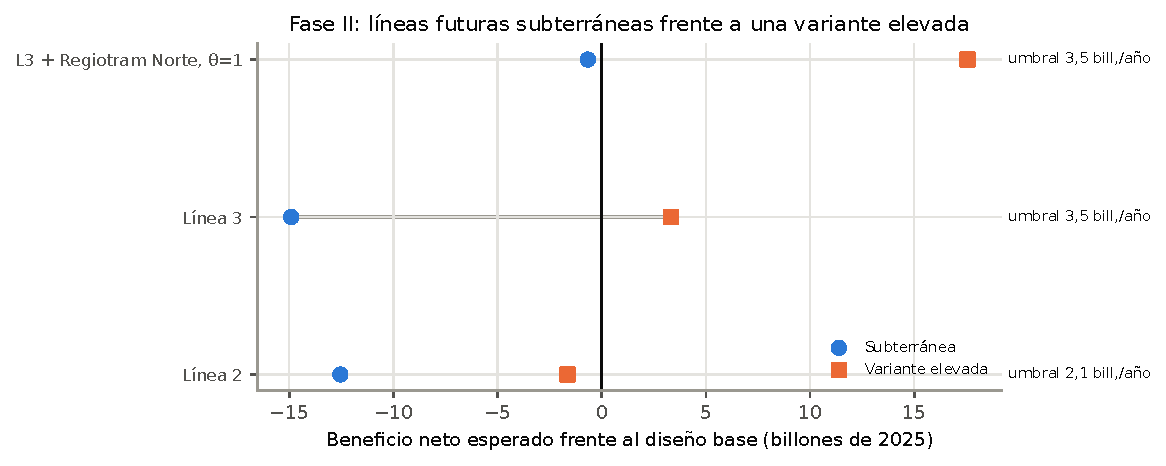
\includegraphics[width=.92\textwidth]{figuras/fig_metro_tipologia.pdf}
\caption{Fase II: beneficio neto esperado de las líneas futuras subterráneas y de sus variantes
elevadas.}\label{fig:metro_tipologia}
\end{figure}

La Línea 2 subterránea tiene un beneficio neto esperado de \BNTipoLdos{} billones y su variante
elevada de \BNTipoLdosE; para la Línea 3, \BNTipoLtres{} y \BNTipoLtresE. Para que el subterráneo
fuera preferible, el viaducto tendría que imponer un costo urbano de \UmbralTipoLdos{} billones por año
en la Línea 2 y de \UmbralTipoLtres{} en la Línea 3, entre diez y veinte veces la estimación por
pérdida de valor de los predios. Un resultado llamativo es que la Línea 3 elevada, combinada con el
Regiotram del Norte y la política de suelo, supera al diseño óptimo de la fase II: su beneficio neto
esperado es de \BNTipoLtresERTN{} billones, frente a \BNTipoRTNTheta{} sin la Línea 3, y además reduce
el CVaR, aunque con una probabilidad de beneficio positivo menor (\PBNTipoLtresERTN{} frente a
\PBNTipoRTNTheta). Con la Línea 3 subterránea, la misma combinación tiene un beneficio neto esperado de
\BNTipoLtresRTN{} billones. Esta comparación supone que existe un corredor donde el viaducto es
viable sin grandes compras de predios; donde no lo hay, el costo del elevado sube y la ventaja se
reduce.

\section{¿Y el tamaño de Bogotá?}

\paragraph{Demanda.} La capacidad no es lo que separa a las dos tipologías. El elevado de la Línea 1
tiene una capacidad de 72.000 pasajeros por hora y sentido \citep{semana2017}; la proyección de 2014 de
81.000 pasajeros por hora y sentido en 2050 \citep{fdn2015} se hizo con una población un millón mayor
que la censada en 2018 y antes de la pandemia. En el modelo, el subterráneo reduce algo más el tiempo
de viaje (\cref{tab:fase2013}), sobre todo porque llega más al norte y tiene más estaciones, pero esa
ganancia no compensa su mayor costo salvo con tasas de descuento bajas.

\paragraph{Tejido urbano.} Es el argumento más sólido a favor del subterráneo, y el que más ha crecido
con el ingreso \citep{ahlfeldt2019}. Pero, para inclinar la decisión de la Línea 1 con la tasa de la
época, el costo urbano del viaducto tendría que ser varias veces mayor que lo que sugiere la pérdida de
valor de los predios; con la tasa actual y el costo oficial de 2014, en cambio, basta con un valor
dentro del rango estimado.

\paragraph{Red.} Esta lectura del tamaño juega en contra del subterráneo. Una ciudad de casi ocho
millones de habitantes y una región que crece necesitan varias líneas, y con un presupuesto limitado
cada kilómetro subterráneo cuesta \KmPorKm{} kilómetros elevados. La fase II muestra que, a la tasa de
9\,\%, las líneas subterráneas adicionales no se pagan, mientras que la política de suelo, el Regiotram
del Norte y una Línea 3 elevada sí. Muchas metrópolis grandes combinan tramos elevados, a nivel y
subterráneos según el corredor; el tamaño de la ciudad no dicta una tipología única.

\section{Conclusiones sobre el metro}\label{sec:conclusiones_metro}

\begin{enumerate}
\item \textbf{Con la información y la tasa de descuento de la época, el metro elevado era la decisión
      con mayor beneficio social esperado.} En la evaluación \emph{ex ante} con 12\,\%, el elevado
      tiene un beneficio neto de \BNElevDoce{} billones frente a \BNSubOfDoce{} del subterráneo con su
      costo oficial y \BNSubUnDoce{} con costos de mercado.
\item \textbf{Esa conclusión no es robusta a la tasa de descuento.} Con la tasa actual de 9\,\% y el
      costo oficial de 2014, las dos tipologías prácticamente empatan, y por debajo de \TasaEmpate{} el
      subterráneo de 2014 sería mejor. Quien sostenga que la Línea 1 debió ser subterránea tiene un
      argumento técnico si acepta el costo oficial de 2014 y una tasa de descuento baja.
\item \textbf{El tamaño de Bogotá, por sí solo, no justifica el subterráneo.} La capacidad del viaducto
      no es la restricción, y la necesidad de una red de varias líneas favorece la tipología que permite
      construir más kilómetros con el mismo presupuesto.
\item \textbf{El costo urbano del viaducto es el argumento decisivo, y es cuantificable.} Con la tasa de
      12\,\% tendría que superar \UmbralOfDoce{} billones por año (costo oficial) o \UmbralUnDoce{}
      (costos de mercado); con 9\,\% y costo oficial, \UmbralOfNueve. Una estimación por pérdida de
      valor de los predios da entre 0,06 y 0,28 billones por año.
\item \textbf{Con lo que realmente ocurrió, el subterráneo habría sido peor.} Con la demanda observada
      y la tasa de 12\,\%, el elevado con apertura en 2028 pierde \BNExpostElevReal{} billones frente a no
      haber construido metro y el subterráneo de costo oficial entre \BNExpostSubDosMilTreinta{} y
      \BNExpostSubDosMilVeinticuatro{} según su fecha de apertura.
\item \textbf{Para las líneas 2 y 3, la elección subterránea exige una justificación explícita.} Cuesta
      entre \AhorroLdos{} y \AhorroLtres{} billones más que una variante elevada, y solo se justifica
      donde el corredor no admite un viaducto o donde el costo urbano es excepcionalmente alto. Una
      Línea 3 elevada entraría en el diseño óptimo de la fase II; la subterránea no.
\item \textbf{Reabrir la tipología de la Línea 1 no tiene sentido económico.} Con la obra contratada y
      avanzada, soterrar un tramo costaría entre 8 y 17 billones adicionales y retrasaría la operación
      varios años \citep{eltiempo2023,narvaez2023}, y la fase I muestra que los retrasos destruyen
      valor.
\end{enumerate}
